\chapter{Test Cases} \label{6Testing}

This chapter details the reasoning and design of the test cases used in this thesis. To provide a common platform for comparing \gls{ble} and 802.15.4¸ Contiki was ported to a platform supporting \gls{ble} as described in chapter \ref{5bleContiki}. \todo{Section }

\section{Performance Metrics Definition} \label{6Metrics}
The aim of this thesis is to compare the key characteristics of the link layer of BLE and 802.15.4. Note that as explained in \todo{section}, 802.15.4 here means the physical layer of 802.15.4 standard. The 802.15.4 standard \gls{mac} later is not used, rather Null-RDC and ContikiMAC, both with \gls{csma} will be used. In this section the four key performance metrics measured for both the wireless protocols are defined in the context of this thesis.

\paragraph{Data rate}
Data rate at the link layer is defined as the maximum amount of data transmitted per second for a protocol with packets containing the maximum allowed payload for the link layer. The data rate is expressed as both kilobits per second and packets per second.

\paragraph{Latency}
In tests for latency, one node needs data from another node, hence as soon as possible it sends a packet requesting the data from the other node and receives the data. Latency is defined as the time from the `\emph{need for data}' arises to the time the requested data is received.

\paragraph{Reliability}
Two criteria will be used for measuring reliability when two nodes are communicating. \gls{prr} is defined as the ratio of the number of packets successfully received to the number of packets sent, both by the link layer. \gls{pdr} is defined as the ratio of the number of packets delivered to the number of packets sent, by the layer above the link layer in both the sender and receiver. While \gls{prr} measures the reliability of transfer of a single transfer of a packet, \gls{pdr} measures the reliability of the link layer to communicate a packet as seen by the layer above it.

\paragraph{Energy Consumption}
The energy consumption in this project is indirectly measured as the \acrfull{rdc}, which is the ratio of the time for which the radio is switched on to the total time of the experiment. Measuring the energy consumption as \gls{rdc} for different scenarios will be more useful to developers as this information will change little across platforms for the same protocol, whereas the actual energy consumed is reducing with every new platform introduced in the market. The processor time utilized by the protocol stack is not considered as this information could not be extracted from the SoftDevice \glspl{api} and also because of the different processor types in the two platforms (32-bit vs 16 bit). 

\section{Test setup} \label{6TestPlatforms}

\subsection{\gls{ble} platform}
The platform used for \gls{ble} is PCA10000, which is described in section \ref{5nrfPCA}. Since BLE is has an asymmetric architecture, a master device is required to communicate with a slave device. In all the tests the slave device is a PCA10000 board running on Contiki and peripheral BLE stack provided by the SoftDevice \emph{S110}. Depending on the test, the master device varied between either a PCA10000 board or an Android device. When a PCA10000 was used as master device, it ran on bare-metal code with central BLE stack provided by the SoftDevice \emph{S120}.

\subsection{802.15.4 platform}

\begin{figure}[h]
    \centering
    \includegraphics[width=\textwidth]{TmoteSky}
	\caption{TmoteSky platform}
    \label{fig:TmoteSky}
\end{figure}


\section{\acrfull{ht} Test Design} \label{6HTdesign}

\begin{figure}[h]
    \centering
    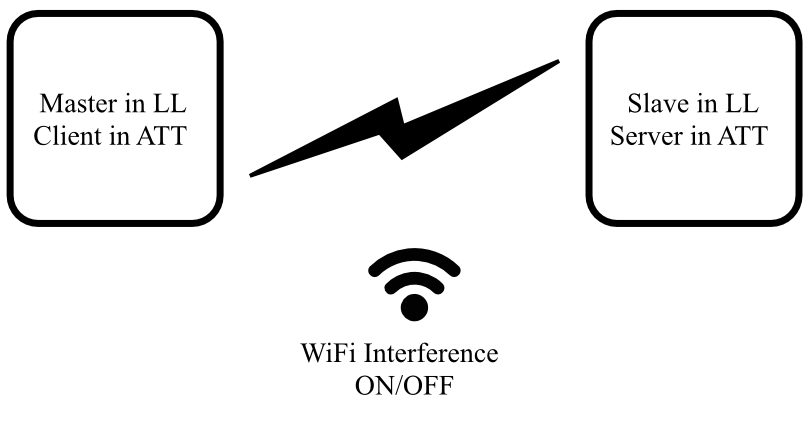
\includegraphics[width=\textwidth]{DataRateSetup}
	\caption{Setup to measure data rate with \gls{ble}}
    \label{fig:DataRateSetup}
\end{figure}

\begin{easylist}[itemize]
& Send packets of maximum size for one minute in the fastest way possible
&& Do one test without CCA for 802.15.4
& Repeat with WiFi
&& Choose a channel interfered by WiFi for 802.15.4 and one channel without WiFi interference.
&& For \gls{ble} do this with channel map with all channels and channel map with WiFi free channels.
& Do this test 10 times
\end{easylist}
\vspace{10pt}


In this test, to measure the various performance criteria in an environment with interference, WiFi interference will be introduced using the tool 'iperf'. The interference pattern generated will simulate streaming of large data over WiFi. \todo{Explain the exact configuration of UDP packets sent}

\vspace{10pt}
Metrics evaluated
\begin{easylist}[itemize]
& Data Rate
& Reliability
& Energy Consumption
\end{easylist}

\section{\acrfull{rr} Test Design} \label{6RRdesign}
\gls{rr} 
\begin{easylist}[itemize]
& Explain what is meant by request response
& Different cases in \gls{ble} and 802.15.4
\end{easylist}

Metrics evaluated
\begin{easylist}[itemize]
& Latency
& Energy Consumption
\end{easylist}


\pagebreak

The objectives of the tests are to compare the link layer of \gls{ble} and 802.15.4 in the aspects mentioned in the following sections. 

The link layer of 802.15.4 consists of \gls{mac} layer on top of a \gls{rdc} layer. For the RDC layer the Null-RDC and ContikiMAC driver will be tested in each of the test with \gls{csma} as the \gls{mac} layer. In case of Contiki-MAC the receiving node switches on periodically to sense if there are any packets that need to be received. The default time of this period is 125 ms. In case of null-RDC the radio receiver is never switched off, as the name suggests.

For \gls{ble}, communication will be done at the Generic Attribute (GATT) layer because the binary from Nordic Semiconductor used in this project does not provide APIs to access the lower layers in both peripheral and central devices. In all the tests the packet structure in 802.15.4 will be same as in \gls{ble} above the link layer.
In this test, to measure the various performance criteria in an environment with interference, WiFi interference will be introduced using the tool 'iperf'. The interference pattern generated will simulate streaming of large data over WiFi. \todo{Explain the exact configuration of UDP packets sent}
In \gls{ble}, the devices can assume different roles in the different layers of the protocol. In the link layer a device can be a 'Master' or a 'Slave'. In the \gls{att} layer, a device can be a 'Client' and/or 'Server'. A server contains data and the client can request data from the server.

In some of the tests, to measure the various performance criteria in an environment with interference, WiFi interference will be introduced using the tool 'iperf'. The interference pattern generated will simulate streaming of large data over WiFi.

\section{Data Rate Test}
This experiment aims to measure the maximum data rate of \gls{ble} and 802.15.4 at the LL with and without WiFi interference. For the \gls{ble} test the devices are configured as shown in the diagram below.

\begin{figure}[h]
    \centering
    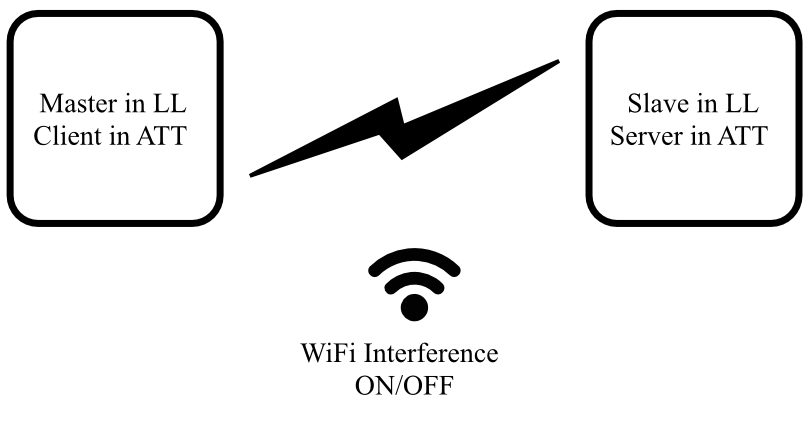
\includegraphics[width=\textwidth]{DataRateSetup}
	\caption{Setup to measure data rate with \gls{ble}}
    %\label{fig:DataRateSetup}
\end{figure}

In this test the data rate is measured by sending data from the server to the client which is not acknowledged in the \gls{att} layer. The data rate is measured at the receiver i.e the Master device. The packet structure will be used such that the complete packet size of \gls{ble} is used. Each run of the test will last of one minute to collect enough data to measure the average data rate.

In case of 802.15.4 one node is configured as transmitter and the other as receiver. The data-rate will be measured at the receiver. In these tests two channels will be used, one which interferes with WiFi and one which does not. This means that each channel will be tested with and without interference. The complete packet size of 802.15.4 will be used when conducting this test.

For data rate measurement tests in both the standards with and without WiFi, the data rate will be measured by sending data for one minute. The data rate will be expressed in both packets per second and \gls{kbps}. 

\subsection{Latency}
This experiment aims to measure the latency for a read request in case of \gls{ble} and 802.15.4, i.e. the time difference between sending the read request packet and receiving the packet with the value requested. In case of both the protocols there are intervals at which the radio is active, where communication can take place. To make sure that the read request packets are sent randomly at any point in this interval, timers with random values would be used to initiate sending these packets. The table below shows the connection parameters used for the various tests to measure the latency with \gls{ble}. The latency is measured at the device sending the packet '1' in the 'Packet' column and is defined as the time from sending the packet '1' to receiving the packet '2'.

\todo{Redo the correct table}


\begin{table}[htbp]
\begin{center}
\begin{tabular}{|l|l|l|l|l|}
\hline
\multicolumn{ 1}{|c|}{\textbf{Connection}} & \multicolumn{ 1}{c|}{\textbf{Connection}} & \multicolumn{ 3}{c|}{\textbf{Devices' Configuration}} \\ \cline{ 3- 5}
\multicolumn{ 1}{|c|}{\textbf{Interval}} & \multicolumn{ 1}{c|}{\textbf{Configuration}} & \multicolumn{ 1}{c}{\textbf{LL}} & \multicolumn{ 1}{|c}{\textbf{GATT}} & \multicolumn{ 1}{|c|}{\textbf{Packet}} \\ \hline
\multicolumn{ 1}{|c|}{} & \multicolumn{ 1}{l|}{Slave latency = 0} & Master & Client & 1. Read request \\ \cline{ 3- 5}
\multicolumn{ 1}{|l|}{} & \multicolumn{ 1}{l|}{
Supervision timeout = 1 \si{\second}} & Slave & Server & 2. Read response \\ \cline{ 2- 5}
\multicolumn{ 1}{|c|}{7.5 \si{\milli\second}} & \multicolumn{ 1}{l|}{Slave latency = 120
} & Master & Client & 1. Read request \\ \cline{ 3- 5}
\multicolumn{ 1}{|l|}{} & \multicolumn{ 1}{l|}{Supervision timeout = 1 \si{\second}} & Slave & Server & 2. Read response \\ \cline{ 2- 5}
\multicolumn{ 1}{|l|}{} & \multicolumn{ 1}{l|}{Slave latency = 120
} & Slave & Server & 1. Indication \\ \cline{ 3- 5}
\multicolumn{ 1}{|l|}{} & \multicolumn{ 1}{l|}{Supervision timeout = 1 \si{\second}} & Master & Client & 2. Indication ACK \\ \hline
\multicolumn{ 1}{|c|}{} & \multicolumn{ 1}{l|}{Slave latency = 0
} & Master & Client & 1. Read request \\ \cline{ 3- 5}
\multicolumn{ 1}{|l|}{} & \multicolumn{ 1}{l|}{Supervision timeout = 1 \si{\second}} & Slave & Server & 2. Read response \\ \cline{ 2- 5}
\multicolumn{ 1}{|c|}{125 \si{\milli\second}} & \multicolumn{ 1}{l|}{Slave latency = 15
} & Master & Client & 1. Read request \\ \cline{ 3- 5}
\multicolumn{ 1}{|l|}{} & \multicolumn{ 1}{l|}{Supervision timeout = 3 \si{\second}} & Slave & Server & 2. Read response \\ \cline{ 2- 5}
\multicolumn{ 1}{|l|}{} & \multicolumn{ 1}{l|}{Slave latency = 15
} & Slave & Server & 1. Indication \\ \cline{ 3- 5}
\multicolumn{ 1}{|l|}{} & \multicolumn{ 1}{l|}{Supervision timeout = 3 \si{\second}} & Master & Client & 2. Indication ACK \\ \hline
\end{tabular}
\end{center}
\caption{\gls{ble} latency measurement test cases}
\label{tbl:testcases}
\end{table}

Where,

\emph{Connection Interval}: After a \gls{ble} connection is established, the master device must always send a packet to the slave periodically after the time specified in connection interval. These connection events provide an opportunity for the slave to communicate with the master.

\emph{Slave Latency}: The maximum number of connection events that a slave can choose not to respond to the master. This is intended to save power on the slave while also providing an opportunity to communicate with the master if necessary.

\emph{Supervision Timeout}: A \gls{ble} connection is said to be lost if there is no bi-directional communication between the master and the slave for the duration specified by supervision timeout. After a tiemout the master will not send a packet to the slave in every connection event.

\emph{\gls{gatt} Read}: A packet containing an (attribute) value sent from a GATT server to a GATT client in response to a request from the client.

\emph{\gls{gatt} Indication}: A packet containing an (attribute) value sent from a GATT server to a GATT client, which the client should acknowledge (ACK). This packet is sent without the client requesting this data.

In the case of 802.15.4, one node is configured to send unicast messages and another is configured to receive these and send a response. The latency using both ContikiMAC and NullRDC will be measured. The latency is measured as the time difference between sending a unicast message and receiving its response.

The \gls{ble} test cases are designed such that the 7.5 \si{\milli\second} tests can compare with Null-RDC test of 802.15.4 while the 125 \si{\milli\second} tests can compare with the  ContikiMAC test of 802.15.4. There are tests with Slave Latency as zero and non-zero, which will help in identifying its effect on latency and the energy consumption of both the master and slave device.

To get an overall sense of the latency over a period of time, the average and standard deviation of the delay for 1000 transactions will be calculated for each test. In all the tests the payload will be of 20 bytes.

\subsection{Energy Consumption}
Energy consumption will be indirectly measured by logging the radio activity in all the tests described above in both the devices communicating. This will provide the duty cycle of when the radio is on. The possibility of logging the sleep cycle of the processor using the binary for \gls{ble} software needs to be verified. If the state of the processor is available, it will also be logged.

\subsection{Reliability}
Similar to measuring the energy consumption, reliability will be evaluated by  correlating the logs of when the radio is switched on versus when the packets are logged. This will provide an idea of how many times a packet has been dropped and hence find out the \gls{pdr}.
